% !TEX root = ../main.tex

\section{The Rust Programming Language} % (fold)
\label{sub:the_rust_programming_language}

Rust \cite{web:rust_lang} is a new open source systems programming language developed by the Mozilla
Foundation \cite{web:mozilla_foundation}. It is designed to support concurrency and parallelism and
take full utilization of the underlying hardware. Rust makes strong guarantees about isolation and
memory safety, while still focusing on performance.

Rust is a strongly and statically typed, multi-paradigm programming language. The language borrows
many traits and features from other, already existing languages. The following subsections discusses
some of the more prominent language features, that all work together in order to achieves Rust's
main goals; mainly full memory safety without sacrificing performance.
\todo{I've just been throwing out ideas and statements that are probably not very true.}

\subsection{Zero-cost Abstractions}
\label{chap:zero_cost_abstractions}

Abstractions, in the form of references and pointers to objects or structures and how they are
structured on the heap, is a common source of overhead in programming languages.
\autoref{fig:java_abstractions} \todo{Update with nicer figure} shows how Java lays out a vector of
strings in memory. A reference to the heap-allocated vector is placed on the stack, and the vector
itself stores internal references to different strings that is placed elsewhere on the heap. Thus,
if the programmer wants to access the first character of a string, two objects have to be found and
dereferenced on the heap in order to read the value;

\begin{enumerate}
  \item the vector must be dereferenced so that a reference to the string can be returned, and
  \item the string must be dereferenced so that character can be read.
\end{enumerate}

If the nesting of objects is deep it can result in many unnecessary heap-lookups in order to get the
desired data.

\begin{figure}[tb]
  \begin{center}
    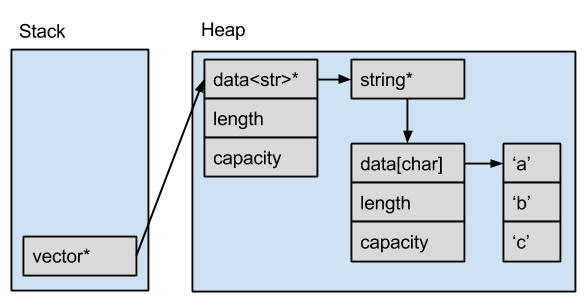
\includegraphics[scale=0.5]{figures/java_abstractions}
  \end{center}
  \caption{Abstractions of a Vector of Strings in Java.}
  \label{fig:java_abstractions}
\end{figure}

Rust introduces the same zero-cost abstractions that are featured in C and C++, among others. This
is both important for performance, and generally in order to have a deterministic and a common
understanding of how the structures are laid out in the memory when working with embedded devices.
\todocite{This is a bogus sentence. Also, need to cite zero-cost abstraction articles}
\autoref{fig:cpp_abstractions} shows how C++ places the structures in memory. The main difference
is that the structure data itself is placed on the stack and inside the vector, instead of the
references to the structures, yet keeping the same level of abstraction. In Rust's case, all
structures is allocated directly on the stack if it is not shared between threads (see the following
paragraphs), allowing for faster data access. This is made possible with a strong notion of variable
ownership in order for the compiler to statically keep track of live stack- and heap-references.
\todo{Don't think this last section is entirely true. Leaving this as a statement for now, that
needs proper backing.}

\begin{figure}[tb]
  \begin{center}
    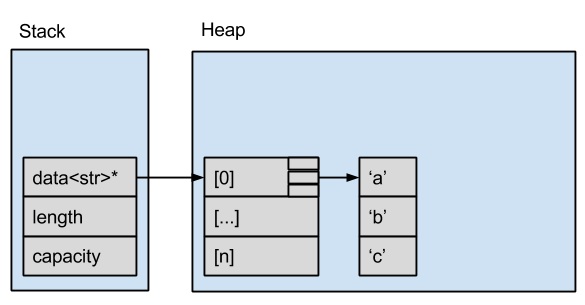
\includegraphics[scale=0.5]{figures/cpp_abstractions}
  \end{center}
  \caption{Abstractions of a Vector of Strings in Rust and C++.}
  \label{fig:cpp_abstractions}
\end{figure}

\subsection{Guaranteed memory safety}

One of Rusts biggest features is full memory safety \cite{web:rust_book_unsafe} without sacrificing
performance. The memory safety boils down to how Rust manages the variables and data-segments
throughout the program. Rust introduces a few concepts that are all centered around the
\emph{ownership} of these variables, how the variables are \emph{borrowed} and the
\emph{lifetimes} of the variables and the borrowed references to them. Rusts ownership system are
part of all the zero-cost abstractions mentioned in \autoref{chap:zero_cost_abstractions}, since all
borrow-checking and ownership- and lifetime-analysis is done statically at compile-time.

\subsubsection{Ownership and Move Semantics} \hfill

In order to achieve full memory safety, we have to remove all form for memory leaks and dangling
pointers to invalid memory. This implies one \emph{memory deallocation} for every respective
\emph{memory allocation}. Traditionally, when allocating memory for a variable, the programming
language will return a \emph{pointer} that is essentially an address to a record in memory,
together with how many bytes it takes to store the record in memory. When there is no longer any
need for the memory it have to be deallocated.

Modern programming languages, like Java and Python, typically achieves this with a Garbage Collector
that runs during program execution with the sole purpose of keeping the memory intact. A common
implementation is a reference counted garbage collector that keeps a count over the number of
references to the variables and deallocates them when there are no valid references to them. The
downside of such an approach to memory safety is the continuous use of resources it requires to keep
track all the references, every assignment and every time the variable enters a scope the reference
count must be increased, and when it leaves a scope it must be decreased.

Another common implementation is a stop-the-world garbage collector. It works differently, by
regularly halting the executing program, and then tracing all references that are accessible from
the root scope and the registers recursively. The memory that are accessible from these references
is then marked as valid, and all the invalid memory will then be freed and accessible through new
calls to memory allocations. The downside of such an approach is the requirement of halting the
entire program in order to release the invalid memory. There are also many other techniques of
garbage collection, that are often a variation of the ones already described, but they are all
troublesome in constraint environments such as found on a small embedded device, or in real-time
systems where the unpredictability of program execution introduced by a garbage collector is
unacceptable.

Another approach to keeping track of the memory resources have been to give the programmer full
control of every memory allocation and deallocation. This is the most common approach for systems
programming languages like C and C++, where performance and predictability is important. However, it
is easier to make the mistakes of referencing invalid memory, or forgetting to free up memory that
might lead the program to use all available resources over time. This will inevitably lead the
program to crash when it tries to allocate more memory when there are no memory left to allocate.

\todo{This subsection about GC and memory handling might be better suited in a different
background chapter}

It is important to always remember and deallocate all memory referenced by a pointer, before the
pointer leaves the scope in the program. Rust operates a little different from C when it comes to
freeing memory, any variables holding a reference to heap-allocated memory will automatically be
freed when it leaves the scope it lives in. This is done statically without the interference of the
programmer. When the compiler sees that the handle for the allocated memory leaves its scope, it
knows that it is lost to the program, so it will insert a call to free the memory at the moment it
leaves the scope and becomes unreachable. This eliminates the need for the programmer to do the
bookkeeping of memory manually. These two aspects of memory allocation and deallocation is combined
into the concept of \emph{ownership} that Rust incorporates. When a handle that \emph{owns} a
reference to a data-segment on the heap leaves its scope, Rust knows that it can safely free the
memory that is referenced by it since it is the \emph{owning handle} of the memory, that can no
longer be used in the program.

\todo[inline]{Show code examples of rust and handle-ownerships}

There can only exist one owned handle to either a heap- or a stack-allocated variable at any time
during program execution. This means that if the handle gets passed as an argument to a function,
this function will take \emph{ownership} of the variable, by \emph{moving} it to the new scope
defined by the function. This move prevents any further use of the handle in its original scope and
is necessary because Rust only allows one handle to a memory-segment at any time. If two or more
handles to the memory had existed at the same time it would have resulted in several calls to
\emph{free}, one for every time the handle left the different scopes. The only way to continue using
the handle in its original scope would have been to give the ownership back after using it.

\subsubsection{Borrowing} \hfill

\emph{Borrowing} is introduced as an alternative to moving the variable ownership across multiple
scopes. Rust allows the programmer to \emph{lend} away access to handles by passing a reference to
the variable around instead of the actual handle itself. There can exist multiple \emph{references}
to the same place in memory, as long there is only one \emph{owner} of the handle itself. A
reference is denoted with an \texttt{\&} in front of the handle, this will tell Rust that we're
working with a reference to the handle, or just borrowing the handle to the end of the active scope.

\todo[inline]{Show code examples of borrowing and references}

\subsubsection{Lifetimes} \hfill

Rust needs a way to ensure that the memory used by all borrowed references to a handle is intact,
i.e. that the references does not point to any deallocated memory. Rust achieves this with a concept
called \emph{lifetimes}, in which  the compiler with the help of \emph{lifetime elisions}, can
statically resolve any dangling pointers or \emph{use-after-free} issues introduced by the
programmer.

Lifetime elisions is applied to structures and function definitions, among others, in order to tell
Rust that the lifetime

\todo[inline]{Show code examples of lifetimes}

\todo[inline]{I have mixed the use of data-segments, variables, pointers and handles. They should be
properly defined and used within the right contexts.}

\subsection{Big-Stack allocation}
\label{par:big_stack}

Rust uses "big stack" allocations \todocite{need big-stack citation. I've read about it somewhere}
and does a good job of avoiding dynamic heap allocation of data. Combined with Rust's strong
lifetime semantics, it is possible to write larger programs that are fully stack-allocated, with
little or no dynamic heap allocations. This can significantly boost performance as the need for
garbage collectors and other runtime requirements is minimal (important for embedded devices).

\todo{Just rambling along to get an idea of something to write.}

% subsubsection memory_safety (end)

\subsection{Concurrency Model} % (fold)
\label{ssub:concurrency_model}

Rust has a concurrency model. Duh.

% subsubsection concurrency_model (end)



% subsection the_rust_programming_language (end)
